\let\negmedspace\undefined
\let\negthickspace\undefined
%\documentclass[journal,12pt,twocolumn]{IEEEtran}
\documentclass[10pt]{article}
\usepackage{cite}
\usepackage{amsmath,amssymb,amsfonts,amsthm}
\usepackage{algorithmic}
\usepackage{graphicx}
\usepackage{textcomp}
\usepackage{xcolor}
\usepackage{txfonts}
\usepackage{listings}
\usepackage{enumitem}
\usepackage{mathtools}
\usepackage{gensymb}
\usepackage{tfrupee}
%\usepackage[breaklinks=true]{hyperref}
%\usepackage{tkz-euclide} % loads  TikZ and tkz-base
%\usepackage{listings}
%\usepackage{gvv}
%\usepackage{setspace}
%\usepackage{gensymb}
%\doublespacing
%\singlespacing
%\usepackage{graphicx}
%\usepackage{amssymb}
%\usepackage{relsize}
%\usepackage[cmex10]{amsmath}
%\usepackage{amsthm}
%\interdisplaylinepenalty=2500
%\savesymbol{iint}
%\usepackage{txfonts}
%\restoresymbol{TXF}{iint}
%\usepackage{wasysym}
%\usepackage{amsthm}
%\usepackage{iithtlc}
%\usepackage{mathrsfs}
%\usepackage{txfonts}
%\usepackage{stfloats}
%\usepackage{bm}
%\usepackage{cite}
%\usepackage{cases}
%\usepackage{subfig}
%\usepackage{xtab}
%\usepackage{longtable}
%\usepackage{multirow}
%\usepackage{algorithm}
%\usepackage{algpseudocode}
%\usepackage{enumitem}
%\usepackage{mathtools}
%\usepackage{tikz}
%\usepackage{circuitikz}
%\usepackage{verbatim}
%\usepackage{tfrupee}
%\usepackage{stmaryrd}
%\usetkzobj{all}
%    \usepackage{color}                                            %%
%    \usepackage{array}                                            %%
%    \usepackage{longtable}                                        %%
%    \usepackage{calc}                                             %%
%    \usepackage{multirow}                                         %%
%    \usepackage{hhline}                                           %%
%    \usepackage{ifthen}                                           %%
  %optionally (for landscape tables embedded in another document): %%
%    \usepackage{lscape}
%\usepackage{multicol}
%\usepackage{chngcntr}
%\usepackage{enumerate}
%\usepackage{wasysym}
%\documentclass[conference]{IEEEtran}
%\IEEEoverridecommandlockouts
% The preceding line is only needed to identify funding in the first footnote. If that is unneeded, please comment it out.
%\newtheorem{theorem}{Theorem}[section]
%\newtheorem{problem}{Problem}
%\newtheorem{proposition}{Proposition}[section]
%\newtheorem{lemma}{Lemma}[section]
%\newtheorem{corollary}[theorem]{Corollary}
%\newtheorem{example}{Example}[section]
%\newtheorem{definition}[problem]{Definition}
%\newtheorem{thm}{Theorem}[section]
%\newtheorem{defn}[thm]{Definition}
%\newtheorem{algorithm}{Algorithm}[section]
%\newtheorem{cor}{Corollary}
%\newcommand{\BEQA}{\begin{eqnarray}}
%\newcommand{\EEQA}{\end{eqnarray}}
%\newcommand{\define}{\stackrel{\triangle}{=}}
%\theoremstyle{remark}
%\newtheorem{rem}{Remark}
%\bibliographystyle{ieeetr}
%\begin{document}
%\bibliographystyle{IEEEtran}
%\vspace{3cm}
%\renewcommand{\thefigure}{\theenumi}
%\renewcommand{\thetable}{\theenumi}
%\renewcommand{\theequation}{\theenumi}
%\begin{figure}
%\centering
%\includegraphics[width=\columnwidth]{./figs/tri_sss.pdf}
%\caption{Triangle generated using python}
%\label{fig:tri_sss_py}
%\end{figure}
%\item Fig. \ref{fig:tri_sss_tikz} is generated using
%\begin{lstlisting}
%math/figs/tri_sss_alone.tex
%\end{lstlisting}
%\begin{figure}[!ht]
        %\begin{center}
        %\resizebox{\columnwidth}{!}{\input{./figs/tri_sss.tex}}
        %\end{center}
        %\caption{Triangle generated using \LaTeX Tikz.}
        %\label{fig:tri_sss_tikz}
%\end{figure}
%\end{enumerate}
%\end{document}
\begin{document}
\title{LATEX ASSIGNMENT}
\author{ANAND}
\date{17-08-2023}
\maketitle
\section*{EXERCISE 9.4.2}
%x\begin{enumerate}
\begin{enumerate}[label=\arabic*.,ref=\theenumi]
\item Draw the graph of each of the following linear equations in two variables:
\begin{enumerate}[label=(\roman*),ref=\theenumi]
\item $x+y=4$
\item $x-y=2$
\item $y=3x$
\item $3=2x+y$
\end{enumerate}
\item Give the equations of two lines passing through (2,14).How many more such lines are there and 
why?
\item If the point(3,4) lies on the graph of the equation $3y=ax+7$ find the value of a
\item The taxi fare in the city is as follows:for te first kilometre,the fare is \rupee~8 and for the 
subsquent distance is \rupee~5 per km.Taking the distance Covered as $x$ km and total fare as
\rupee~y.Write a linear equation for this information,and draw its graph.
\item From the choices given below,choose the equation whose graphs are given Fig 4.6 Fig 4.7
\\
For fig $4.6$ 
\begin{enumerate}[label=(\roman*)]
\item $y=x$
\item $x+y=0$
\item $y=2x$
\item $2+3y=7x$
\end{enumerate} 
For fig $4.7$
            \begin{enumerate}[label=(\roman*)]
\item $y=x+2$
\item $y=x-2$
\item $y=-x+2$
\item $x+2y=6$
\end{enumerate}
\begin{figure}[ht]
\centering
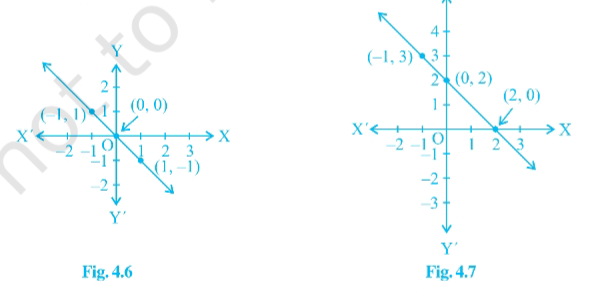
\includegraphics[width=\columnwidth]{4.6&4.7.png}
\caption{Graph}
  \label{fig:Figure}
\end{figure}
\item If the work done by a body of a constant force is directly proportional 
to the distance travelled by the body,express this in the form of an equation
and draw the graph of the same by taking the varables and draw the graph of 
the same by taking the constant force as $5 units$.Also read from the graph the
work done when the distance travelled by the body is
\begin{enumerate}[label=(\roman*)]
\item $2$Units
\item $0$Unit
\end{enumerate}
\item Yamini and Fatima,two students of class IX of a school,together
 contributed \rupee~100 towards the prime minister's reief fund to help
 the earhquake victims.Write a linear equation which satisfies this data.
 (you may take their contributions  \rupee~x and \rupee~y.Draw the graph 
 of the same.
\item In Countries like USA and Canada temperature is measured in Celsius.
Here is a linear equation that converts Farenheit to celsius:
$F=\frac{9}{5}C+32$
\begin{enumerate}[label=(\roman*)]
\item Draw the graph of the linear equation above using Celsius for $x$
 axis and Farenheit for $y$ axis
\item If the temperature is $30\degree C$,what is the temperature in farenheight?
\item If the temperature is $95\degree F$,what is the temperature in celsius?
\item If the temperature is $0\degree C$.What is the temperature in Farenheit and if the temperature in celsius?
\item Is there a temperature Which is numerically same in both Farenheit and Celsius? If yes find it.
\end{enumerate}
\end{enumerate}
\end{document}
